\section{Team Introduction}

We are Sooner Competitive Robotics (SCR) at the University of Oklahoma. Our organization has existed since 2013, and we have competed all over the U.S. since then. We intended to participate in the IGVC AutoNav challenge in 2020, but since it was canceled, this will be our first time competing. 

Our robot is called the Aluminium Whale. Last year, our chassis was a heavy steel frame that we struggled to push and carry around, so we called it the Steel Cannon. This year, we used aluminum for our main frame, with most paneling being acrylic, so the robot is much lighter. When doing our first outdoor drive test, we found that our clearance between the underside of the base and the ground was so small that the robot could easily become ``beached'' on the edges of sidewalks or even small perturbations in the height of the dirt. This led us to a name within the same naming scheme as its predecessor, the Aluminum Whale. (We've improved our clearance since then, so we hope this namesake will not be demonstrated during the competition). 

\begin{figure}[h]
    \centering
    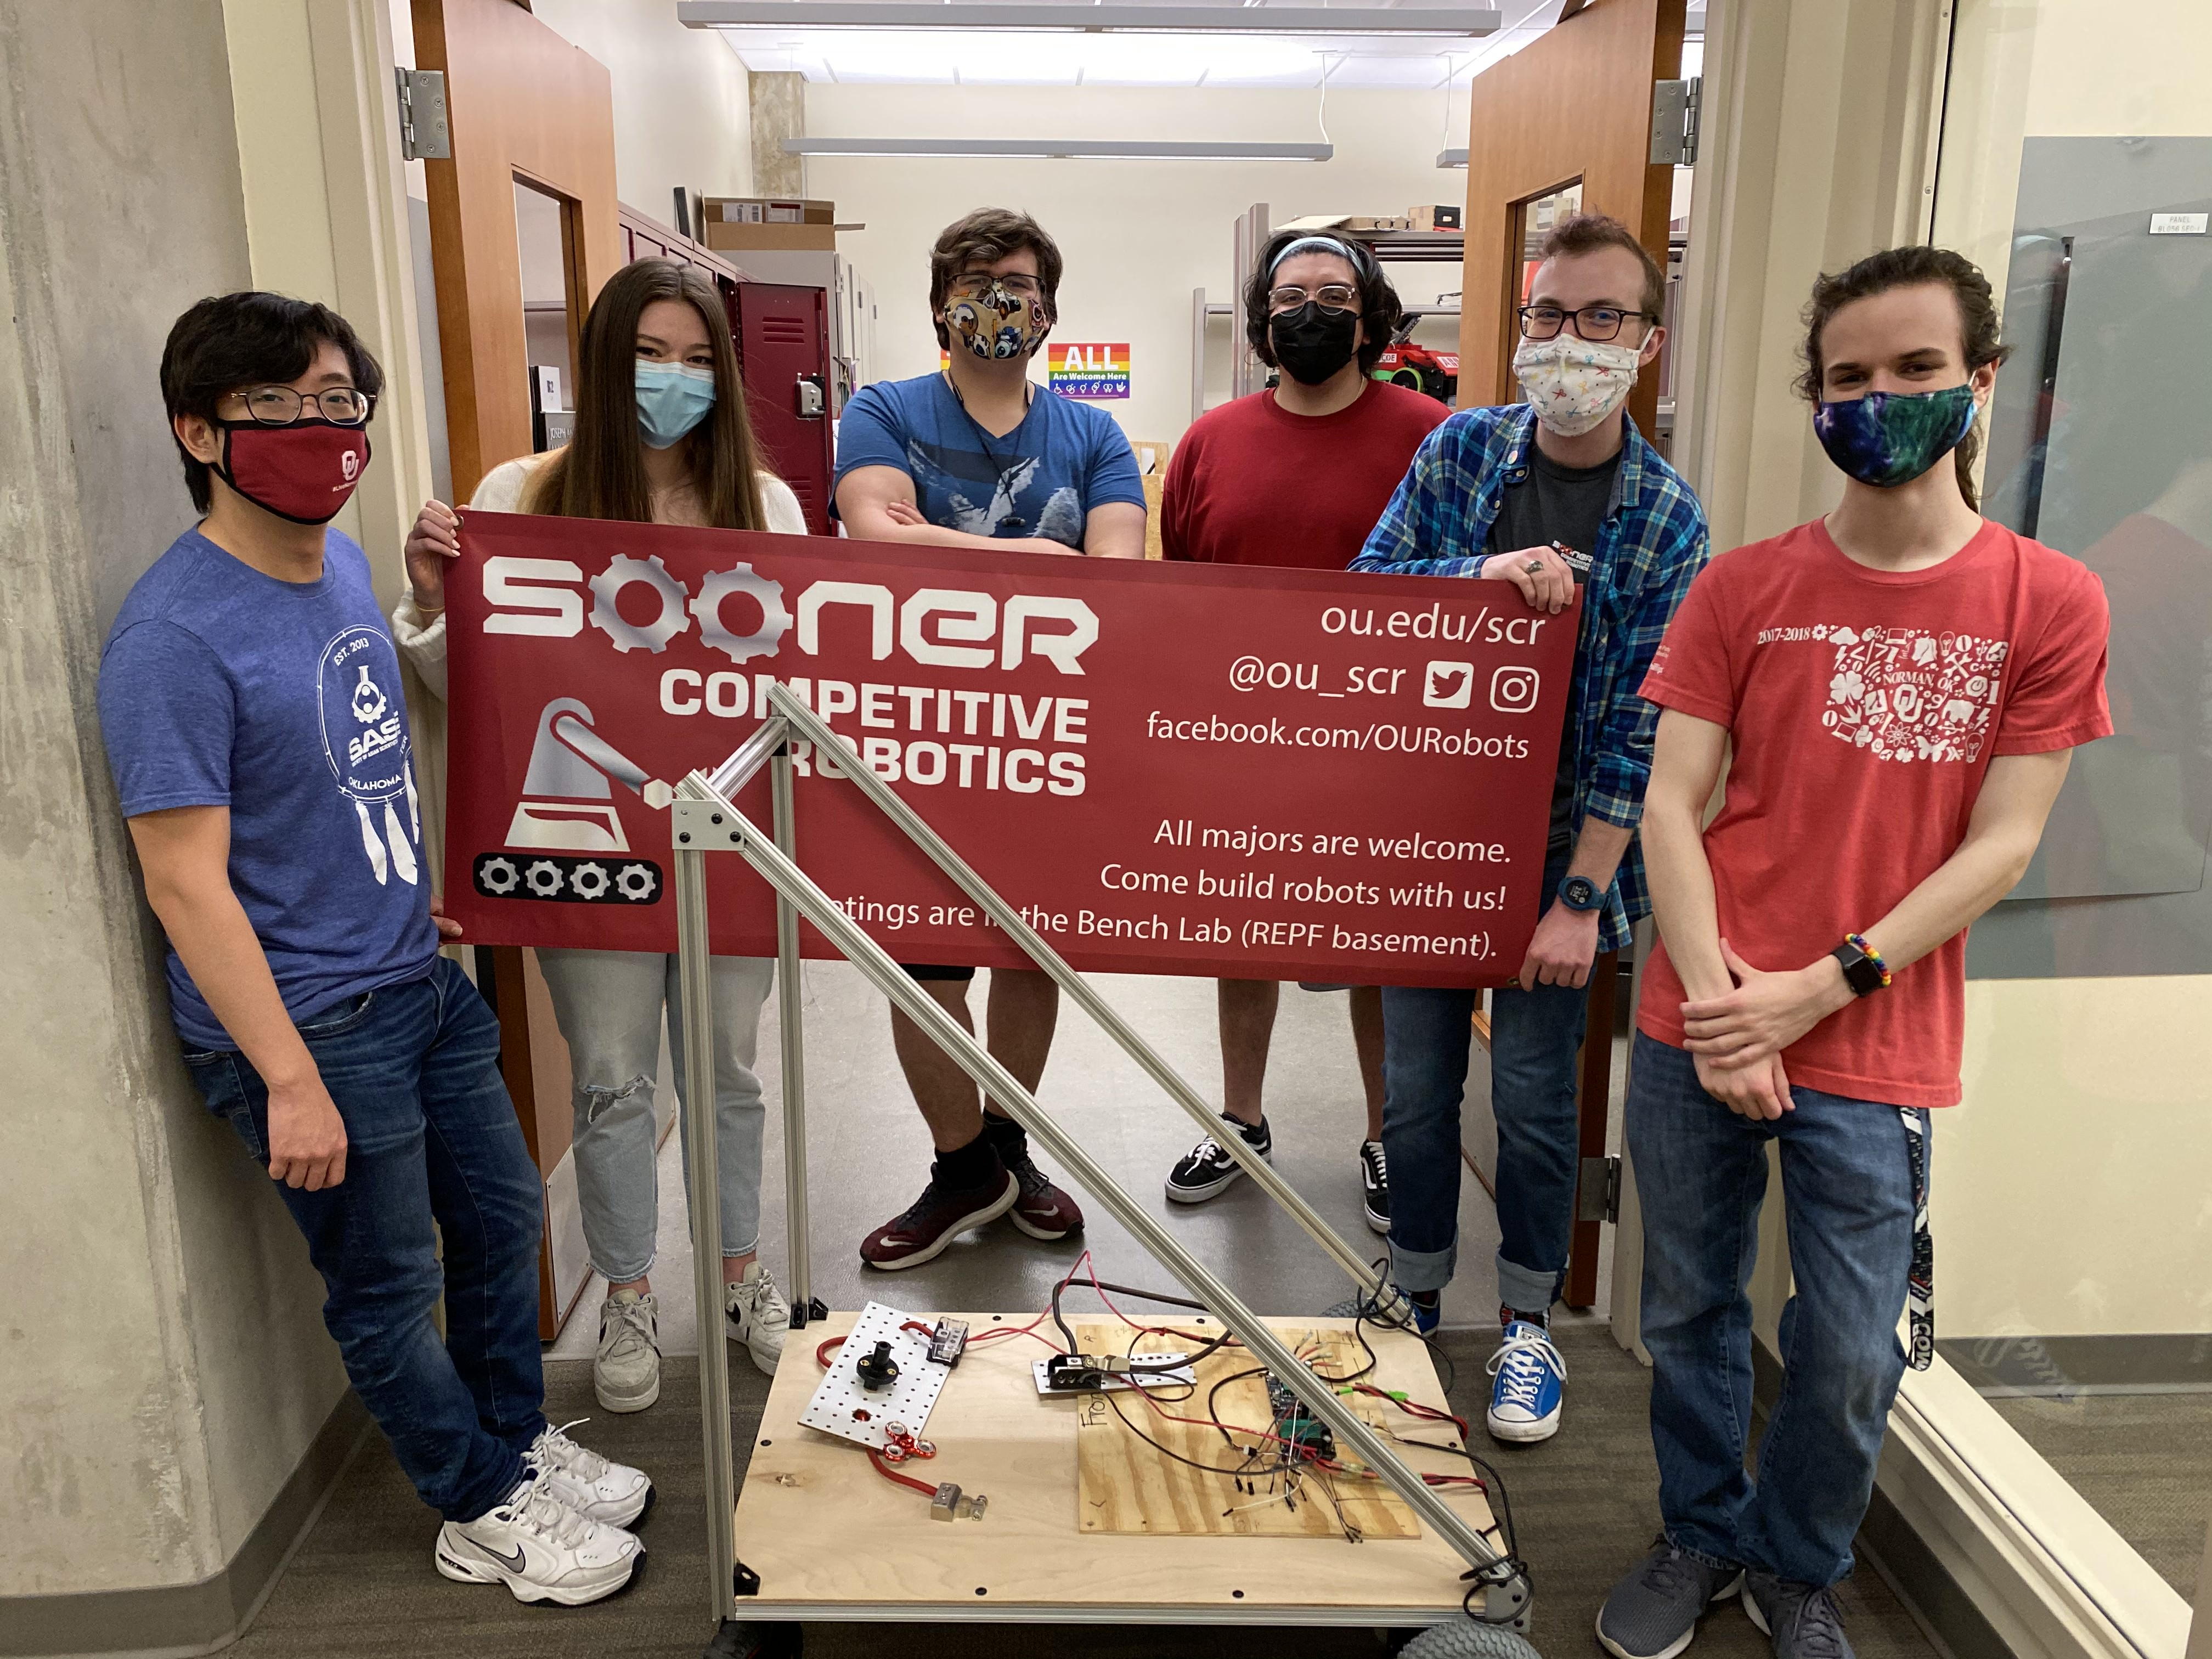
\includegraphics[width=0.5\textwidth]{images/team.jpg}
    \caption{The team with an early version of the robot.}
\end{figure}

The team was organized into three subteams (software, electrical, and mechanical), but membership on these teams was not mutually exclusive. Since our team is so small, many of our members contributed to multiple areas throughout our build process. The following table shows each member with their area(s) of contribution (S=Software, E=Electrical, M=Mechanical). 

\begin{center}
\begin{tabular}{|c c|}
    \hline
    Kevin Robb & S/M \\
    Noah Zemlin & S/E/M \\
    Tyler Julian & E/M \\
    Jorge Exinia & E/M \\
    Kichang Song & S \\
    Sarah Brown & E \\
    Stephanie Sheldon & M \\
    \hline
\end{tabular}
\end{center}

We identify Software contributions as significant work towards the code for part of the robot’s autonomous operation or other functionality.  Firmware creation is classified under Electrical. Work with PCB design, wire routing, and everything else in that realm falls under Electrical. Mechanical work includes design and construction of the main robot, 3D modeling, and printing of mounts and other parts, and considerations such as robot leveling, squaring, and weight distribution.

